\newpage
{\bfseries МРНТИ 52.47.01}
\hfill {\bfseries \href{https://doi.org/10.58805/kazutb.v.2.23-431}{https://doi.org/10.58805/kazutb.v.2.23-431}}

\sectionwithauthors{B. Nuranbayeva}{THE FEASIBILITY STUDY ON EFFICIENCY OF DEVELOPMENT OF THE OIL FIELD ON THE LAND AND THE SHELF OF THE CASPIAN SEA WITH USE GRAVITATIONAL MODE OF PRODUCTION}

\begin{center}
{\bfseries B. Nuranbayeva}

Caspian University, Almaty, Kazakhstan,

{\bfseries \textsuperscript{🖂}}Corresponding author: bulbulmold@mail.ru
\end{center}

Traditional technologies of oil production on the land and the sea shelf
have low coefficient of oil recovery, thus cause a huge loss to
environment to what become frequent oil spills testify worldwide. In
article the innovative way of development of oil fields allowing to
increase significantly oil recovery by means of artificially created
gravitational mode is described and also completely to exclude
environmental pollution when developing offshore fields thanks to oil
production by a dense grid of wells which are drilled from horizontal
wells. In comparison with usual ways of oil production on the shelf,
such as development, from bulk islands, oil platforms and platforms,
this way has a number of technological and economic advantages.
Experience of application of similar technologies around the world is
considered. For comparison outputs of wells and capital expenditure on
the example of oil fields Kyrykmyltyk and Kashagan in Kazakhstan are
counted.

{\bfseries Keywords:} oil, well, development, shelf, bulk island,
efficiency, gravitation.

\begin{center}
{\large\bfseries ШАХТА-ҰҢҒЫМА ТӘСІЛІН ПАЙДАЛАНА ОТЫРЫП КАСПИЙ ТЕҢІЗІНІҢ
ҚАЙРАҢЫНДАҒЫ ҚАШАҒАН МҰНАЙ КЕН ОРНЫН ИГЕРУ ТИІМДІЛІГІНІҢ}

{\bfseries ТЕХНИКАЛЫҚ-ЭКОНОМИКАЛЫҚ НЕГІЗДЕМЕСІ}

{\bfseries Б.М. Нұранбаева}

Caspian University, Алматы, Қазақстан,

e-mail: bulbulmold@mail.ru
\end{center}

Құрлықта және теңізде шельфтегі дәстүрлі мұнай өндіру технологиялары
қоршаған ортаға орасан зор зиян келтіре отырып, мұнай өндірудің төмен
коэффициентіне ие, бұл бүкіл әлем бойынша мұнайдың жиі төгілуінен
көрінеді. Мақалада жасанды түрде жасалған гравитациялық режим арқылы
мұнай өндіруді едәуір арттыруға, сондай-ақ көлденең ұңғымалардан
бұрғыланатын ұңғымалардың тығыз торымен мұнай өндіру арқылы Теңіз кен
орындарын игеру кезінде қоршаған ортаның ластануын толығымен жоюға
мүмкіндік беретін мұнай кен орындарын игерудің инновациялық әдісі
сипатталған. Үйінді аралдардан, мұнай платформаларынан және
платформалардан игеру сияқты қайраңда мұнай өндірудің әдеттегі
әдістерімен салыстырғанда, бұл әдіс бірқатар технологиялық және
экономикалық артықшылықтарға ие. Әлемде осындай технологияларды қолдану
тәжірибесі қарастырылды. Салыстыру үшін Қазақстандағы Қырықмылдық және
Қашаған мұнай кен орнының мысалында ұңғымалардың дебиттері мен күрделі
шығындар есептелді.

{\bfseries Түйін сөздер}: Мұнай, ұңғыма, игеру, шельф, үйінді арал,
тиімділік, ауырлық күші.

\begin{center}
{\large\bfseries ТЕХНИКО-ЭКОНОМИЧЕСКОЕ ОБОСНОВАНИЕ ЭФФЕКТИВНОСТИ РАЗРАБОТКИ
НЕФТЯНГО МЕСТОРОЖДЕНИЯ КАШАГАН НА ШЕЛЬФЕ КАСПИИЙСКОГО МОРЯ С
ИСПОЛЬЗОВАНИЕМ ШАХТНО-СКВАЖИННОГО СПОСОБА}

{\bfseries Б.М. Нуранбаева}

Caspian University, Алматы, Казахстан,

e-mail: bulbulmold@mail.ru
\end{center}

Традиционные технологии добычи нефти на суше и морском шельфе имеют
низкий коэффициент нефтеотдачи, при этом наносят огромный ущерб
окружающей среде, о чем свидетельствуют частые разливы нефти по всему
миру. В статье описан инновационный способ разработки нефтяных
месторождений, позволяющий значительно увеличить нефтеотдачу за счет
искусственно созданного гравитационного режима, а также полностью
исключить загрязнение окружающей среды при разработке морских
месторождений за счет добычи нефти плотной сеткой скважин, которые
бурятся из горизонтальных стволов. По сравнению с обычными способами
добычи нефти на шельфе, такими как разработка, с насыпных островов,
нефтяных платформ и платформ, этот способ имеет ряд технологических и
экономических преимуществ. Рассмотрен опыт применения подобных
технологий в мире. Для сравнения подсчитаны дебиты скважин и капитальные
затраты на примере нефтяных месторождений Кырыкмылтык и Кашаган в
Казахстане.

{\bfseries Ключевые слова:} нефть, скважина, разработка, шельф, насыпной
остров, эффективность, гравитация.

\begin{multicols}{2}
{\bfseries Introduction.} The oil and gas industry in Kazakhstan has
traditionally been regarded as the leading activity that determines the
main trends of economic development and growth in the country and has
one of the greatest impacts on the welfare of Kazakhstanis. This state
of affairs is explained by the presence of large oil and gas reserves in
Kazakhstan, the high level of production of these raw materials in the
country and the corresponding volumes of exports. Thus, according to
various estimates, Kazakhstan\textquotesingle s total oil and gas
reserves are estimated at 11-12 billion tonnes, with daily production of
oil and gas condensate in the country increasing from 0.52 million
barrels (0.7\% of world supply) to 1.97 million barrels (1.9\% of world
supply) between 1997 and 2019. At the same time, from 1999 to 2018, the
volume of Kazakhstan\textquotesingle s oil and gas condensate exports
increased from 47.1 million to 69.8 million tonnes.

Currently, one in four tonnes of oil in the world is recovered from the
seabed. Offshore exploration drilling is taking place in more than 65
countries and covers shelves on all continents. Among them, Saudi
Arabia, Great Britain, Mexico, Venezuela, and the United States are the
countries producing the largest amount of oil offshore.

In recent decades, the share of oil and gas in the world fuel and energy
balance accounts for more than 70 per cent of all energy sources. Taking
into account the high environmental requirements of the public for the
construction of nuclear and hydraulic power plants, it will increase
even more in the future. In connection with this, specialists of oil and
gas industry of all countries faced the problem of search, exploration,
development and exploitation of continental shelf fields, turning it
into a large base of hydrocarbon raw materials, where over 700 million
tonnes of oil and 300 billion m3 of gas are produced annually. Oil and
gas prospecting and exploration works in these zones are carried out in
more than 70 countries, including the Arctic regions of the USA and
Canada. At the same time, the share of oil produced in 45 countries in
the world production volume has already exceeded 28\% and is expected to
increase to 45-65\% (approximately by 2020). Kashagan production in 2023
reached a record level of about 18.8 million tonnes {[}1{]}.

The annual total cost of developing offshore oil and gas resources in
developed and developing countries exceeds \$50 billion. The annual
total cost of offshore oil and gas development in developed and
developing countries exceeds USD 50 billion, of which about 25\% is
spent on prospecting and exploration. For example, more than 60 billion
US dollars were spent on exploration of oil and gas resources in the
British sector of the North Sea alone in 1965-1985, which made it
possible to develop oil and gas resources in the 25 years after the
development of the North Sea. For example, more than \$60 billion was
spent on exploration of oil and gas resources in the British sector of
the North Sea between 1965 and 1985, which made it possible to increase
the level of oil production in the British sector to 124.4 million
tonnes per year within 25 years after the start of the work. This
success was due to the development of a proper strategy for prospecting,
exploration, development, exploitation of the fields in this offshore
region and the construction of the necessary technical means and
facilities for this purpose.

In July 1999, the OKIOC International Consortium began drilling the
first well on the East Kashagan structure using the Sun-Kar drilling
barge. The well is located approximately 75 kilometres south-west of the
city of Atyrau. On 24 July 2000, the well reached a depth of
approximately 5,100 metres and OCIOC officially announced the discovery
of the Kashagan oil and gas field offshore the Caspian Sea. An
oil-bearing interval was discovered in Paleozoic carbonates at a depth
of 4126 m (the interval is 61 m long and the whole oil-bearing formation
is 1026 m) and oil flow rate of up to 600 m\textsuperscript{3} per day
and gas flow rate of 200 thousand m3 per day were obtained. According to
experts, the total reserves of oil and raw materials in the East
Kashagan field are estimated at 7 billion tonnes, and the total of about
100 promising structures of Kazakhstan\textquotesingle s Caspian shelf
at 10-12 billion tonnes.

At present, the international consortium Agip KCO (formerly OKIOC) has
drilled exploration wells on the Kashagan, South-West Kashagan, Aktoty,
Kairan, Kalamkas Sea structures.

Another Kazakhstani offshore project is the development of two nearshore
offshore blocks off the coast of the Kurmangazy and Isatai districts of
the Atyrau region and includes exploration and development of the South
Zhambai pre-salt structure and a number of above-salt structures,
including South Zaburye. The works on these blocks are conducted by NC
KazMunayGas JSC. Recently JSC «Kazakhstankaspiyshelf» completed the
second stage of three-dimensional seismic survey, drilling of an
exploration well is planned.

If all forecasts on oil reserves of Kazakhstan\textquotesingle s part of
the Caspian Sea shelf are confirmed, then in the near future Kazakhstan
can safely count on a place in the seven countries with the largest
crude oil reserves.

The experience of work on offshore oil and gas fields shows that for
their effective development the traditional technical means and methods
used on land are often unacceptable. In order to realise this problem,
especially in connection with the development of the Arctic shelf and
the increase in the depth of the sea, it is necessary to carry out
complex research work and create special technical means and
technologies. The practice of exploitation of the Caspian Sea reservoirs
makes it possible to establish technical, technological and
organisational conditions for the development of offshore deposits, oil
and gas production, rational methods of their intensification, as well
as the main factors ensuring the increase in oil recovery.

For the first time the gravitational way of oil production was applied
in industrial scale in several countries, but didn\textquotesingle t
gain further development, as demanded construction of additional
excavations (tunnels, mines, cross-cuts, etc.) though allows increase
oil recovery of oil fields considerably. The most considerable
industrial facilities {[}2-5{]} where the gravitational mode of
production was applied.

Peshelbronn field in France where due to application of such way oil
recovery increased from 17\% to 43\%.

OnSarata-Monteor field in Romania due to application of the
gravitational mode oil extraction reached 55 -- 60\%.

In 1939 development of the Yaregsky field of a deposit of heavy oil,
with application of excavations and the gravitational mode, allowed to
bring oil recovery to 50 -- 60\% is begun that it is much higher than a
level, reached when developing oil fields of small and average viscosity
by traditional methods.

For development of a field of Troms of II in the Norwegian Sea the
option of replacement of expensive oil platforms with the tunnels gone
from the land on 30 km to side of the sea {[}6{]} was offered.

The given examples show that artificially created gravitational mode
when developing fields of light crude allows reach 60\% of oil
extraction and more. It can be also used for further development of
fields of light crude where traditional ways of oil production sputtered
out.

Today, oil and gas resources are depleted in most onshore oil and
gas-bearing areas, and it is difficult to increase commercial reserves.
In this connection, in recent decades, developed countries have sharply
increased interest in the problem of developing oil and gas resources of
the seas and oceans. The surface of the world ocean accounts for 71\% of
the Earth\textquotesingle s surface, of which 7\% is the continental
shelf, which contains significant potential oil and gas reserves.

\emph{The purpose} of this work to describe and show efficiency of the
new gravitational way of development of fields of light and
high-viscosity crude offered by us on the land and sea the shelf,
excluding shortcomings of earlier known ways.

{\bfseries Methods and Materials.} The northern Caspian Sea contains
important bioresources, including populations of valuable food fishes,
the waterfowl living in a coastal zone, and the most part of population
of the Caspian seals.

Therefore oil operations in this territory should be performed carefully
that there was the minimum impact on fragile ecology and bioresources of
the area of the works which are of great importance for the population
and economy of Kazakhstan and other Caspian states.

The giant Kashagan field is the largest discovery in the last four
decades. Kashagan is one of the most complex industry projects in the
world due to high levels of hydrogen sulphide, harsh offshore
environmental conditions and engineering, logistics and safety issues.

For sea flora and fauna oil spills and emissions can have catastrophic
consequences as it took place in the Gulf of Mexico {[}7{]}. The example
of open emission of oil with gas on a field Tengiz in 1985 is also
instructive. The largest Kashagan field is located on the shelf of the
Caspian Sea has similar geology with Tengiz.

In case of development of a field with application of the gravitational
mode offered by us, the incidents described above are excluded as there
is no contact of the sea with wells.

Thus, no weather conditions, and also a winter season influence oil
production in the gravitational way, and production can be carried out
24 hours per day during the whole year {[}8{]}.

The known technology provides creation of tunnels or other mountain
developments below productive layer from which on this layer drill the
draining trunks. For safety horizontal excavations usually create in the
steady formations below layer providing reliable isolation from oil
layer. In the offered way {[}9{]} the main shortcoming is need of
drilling of the draining wells from below up, i.e. rising that is very
problematic.

Deposits of natural bitumens and heavy oil, the preserved deposits with
high-viscosity oil, the developed fields with considerable residual
reserves of oil and in the long term a zone of a continental shelf
{[}10, 11{]} can be objects of development with application of heat and
forces of gravitation first of all.

{\bfseries Results and Discussion}. For carrying out researches data on
development of such fields in Kazakhstan as Kyrykmyltyk and Kashagan
were used. Thus the method of research including the analysis and
synthesis of known and settlement data is used.

For the purpose of increase of productivity of production wells, oil
recovery of layers, environmental protection and safety of objects of
oil and gas production, the innovative way of their opening and
operation at which artificially created gravitational operating mode of
layer throughout the entire period of operation of a field is provided
is offered below, and on a surface there will be only one well. For this
purpose in the above-lying breeds (roof) layers from a trunk of a
vertical well, horizontal wells through which the field is opened with
the vertical wells constructed underground by their drilling from top to
down from a horizontal well are carried out. For conducting of the
initial vertical well connecting with horizontal to Kashagan it is
offered to use bulk islands of a certain design (fig. 1).

Thus coast of a construction are executed flat and on perimeter are
filled up with shell rock waste, and from above a shell rock
sub-standard waste of production of biologically active mineral minerals
(quartz, bentonite, a shungit, a glaukonit or others) which clear and
improve biological quality of water round the island (fig. 1).

Use of a cylindrical cavity allows to reduce load of an island body when
drilling a vertical and horizontal well that excludes formation of
cracks. Besides, at accidents the flowed-out oil will be isolated from
hit in a cavity of the island and then in the sea and can be pumped out
in special capacity at rescue and recovery operations.

Use of waste of production of biologically active mineral minerals
(quartz, bentonite, a shungit, a glaukonit or others) allows to solve at
the same time a problem of cleaning and improvement of quality of sea
water round the island and recycling of production of a shell rock, and
biologically active mineral minerals (quartz, a shungit, bentonite, a
glaukonit or others).

Thus high technical and ecological reliability of a construction is
provided and it isn\textquotesingle t required considerable material
inputs.
\end{multicols}

\begin{figure}[H]
    \centering
    \begin{subfigure}[b]{0.45\textwidth}
      \centering
      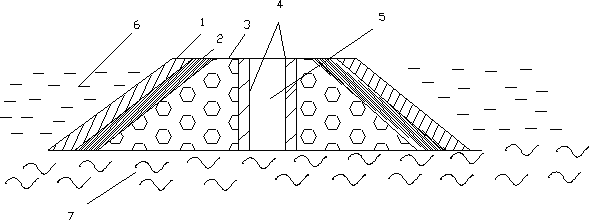
\includegraphics[width=\linewidth]{assets/1339}
    \end{subfigure}
    \begin{subfigure}[b]{0.45\textwidth}
	\caption*{
    1- layer from biologically active breed

    (bentonite, quartz, shungit, glaukonit or other)

    2- layer from a shell rock

    3- soil which is washed up in the course of deepening of the shelf
    or a flood plain of the river

    4-iron or ferroconcrete protections

    5-cylindrical cavity for drilling of wells

    6-sea water

    7- seabed}
    \end{subfigure}
  \caption*{Figure 1- Scheme of a section of the hydraulic engineering construction (the bulk island for oil operations on the shelf)}
\end{figure}

\begin{multicols}{2}
On the shelf over the location of layer of hydrocarbons and where
hydrochloric layer doesn\textquotesingle t stretch, build usually bulk
island \emph{1}, the design {[}12{]} stated above through which pass a
vertical well \emph{2} up to one depth below than a level of the sole of
hydrochloric layer \emph{5}, and also a horizontal well \emph{6} passing
on a roof of layer of hydrocarbons from which drill short operational
wells the 7th diameter of d\textsubscript{1} before crossing with layer
of oil or gas, punch lower than a level of crossing them with layer and
exploit them before the termination of the gushing mode then wells
\emph{7} deepen below layer. To pass to the gravitational mode of
operation well should beadditionally drilled by thechisel of bigger
diameter of d\textsubscript{2} at such length that well volume with a
big diameter of d\textsubscript{2} was more than a volume of a well
diameter of d\textsubscript{1} (fig. 2).
\end{multicols}

\begin{figure}[H]
    \centering
    \begin{subfigure}[b]{0.65\textwidth}
      \centering
      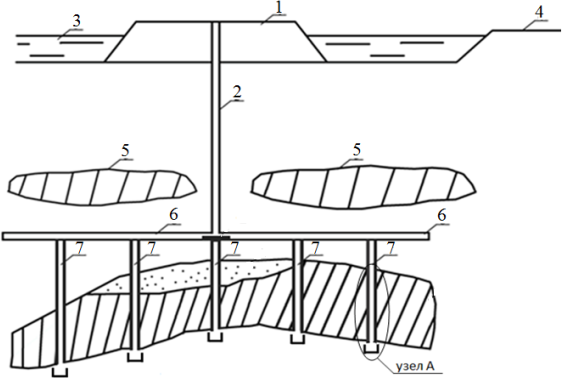
\includegraphics[width=\linewidth]{assets/1340}
      \caption*{Figure 2-Way of opening and operation of oil layers on the shelf and the land}
    \end{subfigure}
    \begin{subfigure}[b]{0.25\textwidth}
      \centering
      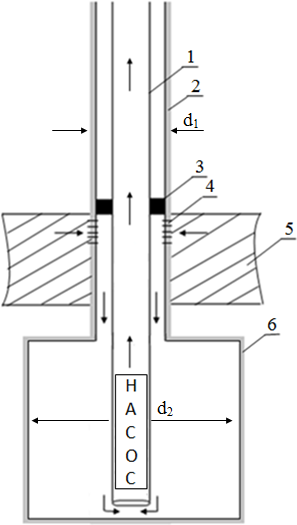
\includegraphics[width=\linewidth]{assets/1341}
      \caption*{Figure 3-Well hub A}
    \end{subfigure}
  \caption*{}
\end{figure}

\begin{multicols}{2}
Thus, at the expense of gravitational force liquid (oil and reservoir
water) will constantly follow from layer in a well with a diameter of
d\textsubscript{2}. From a well diameter of d\textsubscript{2} reservoir
liquid is pumped out by the pump as a result the constant gravitational
operating mode of layer will be provided, and on the bulk island there
will be only one well through which oil and gas will be given. At this
way of opening of layers and oil production well productivity increases,
oil recovery of layers increases, destruction conditions at operation of
wells 2, 6 and 7 since all of them pass not through hydrochloric layer
are eliminated. Also construction of a large number of bulk islands,
allocation of the huge squares at surfaces under drilling of wells
isn\textquotesingle t required, and also length of mining wells 7 is
reduced, pollution of the surrounding and marine environment decreases.
Besides safety of oil objects, including from attacks from air increases
at the military conflicts.

This innovative way of opening and development of a field can be used
not only on the fields which are again opened, but also operating and
fulfilled earlier. Thus it is possible to use more effectively all
existing methods of increase of oil recovery of layers.

Technical and technological and economic calculations of efficiency of
oil production are given below in the offered way (on the example of
fields Kyrykmyltyk and Kashagan).

In technical and technological calculation we consider the Kyrykmyltyk
field a vertical and horizontal well under the horizon of MI -- A where
there is the most viscous oil in comparison with other horizons, a
deposit depth the smallest and the well operating this layer, most a
nizkodebitna concerning other wells.

Basic data on the horizon of MI - A:

- layer depth -- \emph{Н}=300 \emph{m};

- average permeability on layer -- \emph{к}= 1377,4 \emph{mD} =
1377,4⋅10\textsuperscript{-15}\emph{m\textsuperscript{2}};

- density of oil in layer conditions -- \emph{ρ\textsubscript{oil}} =
885,6 \emph{kg/m\textsuperscript{3}};

- effectivepetrosaturated thickness of layer --
\emph{h\textsubscript{effective}} = 11,2 \emph{m};

- average formation pressure -- \emph{Р\textsubscript{layer}} = 2,7
\emph{MPa};

- dynamic viscosity of oil- \emph{µ} = 620 \emph{mPa⋅sec};

- oil-bearing capacity contour radius -- \emph{r\textsubscript{к}}= 1300
\emph{м} (deposit circular, with2,7×2,5 km parameters );

- \emph{r\textsubscript{c}} =
160⋅10\textsuperscript{-3}\emph{м}⋅е\textsuperscript{0,5} =
263⋅10\textsuperscript{-3}\emph{м}.

We choose the radius of a well equal-- \emph{r\textsubscript{c}}=
160⋅10\textsuperscript{-3}\emph{м}⋅е\textsuperscript{0,5}=
263⋅10\textsuperscript{-3}\emph{м}(from practical and theoretical data).
The construction of a vertical site of a well goes up to the depth of
400 m that is depths of the productive horizon interesting us are 100 m
lower. Length of the horizontal site of a well passed from a trunk of a
vertical well along layer is equal 1500 m, that is the construction goes
to the middle of a deposit as we conduct calculations only for one
skilled well located on the center of a deposit. At further development
with increase in number of wells on a deposit length of a horizontal
site of a well can be extended, up to length of all deposit.

In the calculations given below it is shown increase in an output of a
well and respectively a coefficient of oil recovery of layer at the
scheme of its opening stated above. As the well is located on the center
of a deposit and thus there is a plainly radialfiltration of liquid, we
have the right to use a basic formula of Dupuis for calculation of an
output of a well. Originally it has an appearance:

\begin{equation}
Q=V*S
\end{equation}

where\emph{V} -- liquid filtration speed,

\emph{S} -- area of cross section of a well.

Speed of the V filtration of liquid and the area of S can be presented
as:

\begin{equation}
  V = \frac{\kappa}{\mu} \cdot \frac{\partial P}{\partial r} = \frac{\kappa}{\mu} \cdot \frac{P_{\text{пл}} - P_{\text{с}}}{\ln \left( \frac{r_{\text{k}}}{r_{\text{c}}} \right)} \cdot \frac{1}{r_{\text{c}}}
\end{equation}

\begin{equation}
S = 2\pi r_{\text{c}} h
\end{equation}

Therefore, substituting (2) and (3) in a formula (1) we receive a final
formula of Dupuis:

\begin{equation}
Q = \frac{2 \pi \kappa h}{\mu} \cdot \frac{P_{\text{пл}} - P_{\text{c}}}{\ln \left( \frac{r_{\text{k}}}{r_{\text{c}}} \right)}
\end{equation}

For Dupuy\textquotesingle s formula offered innovative technology
assumes some other air. At usual operation of wells pressure in a well
is equivalent to pressure on a face of a well and it to equally
hydrostatic pressure of a column of liquid which creates
counter-pressure on layer, $P_{\text{c}} = \rho g h$
The main idea of our innovative development is that we have no pressure
of a hydrostatic column of liquid, i.e. Rc=0, isn\textquotesingle t
present counter-pressure on layer for the reason that oil under positive
action of gravitation goes down, but not up as at usual operation.

Thus, we receive a modified formula of Dupuis for our technological
conditions which can be presented as:

\begin{equation}
Q = \frac{2 \pi \kappa h}{\mu} \cdot \frac{P_{\text{пл}}}{\ln \left( \frac{r_{\text{k}}}{r_{\text{c}}} \right)}
\end{equation}

Owing to perforation of a well, we receive hydrodynamic - imperfect
system on nature of opening. Therefore, in calculations we take the
specified well radius. It is equal:

\begin{equation}
r_{\text{спр}} = r_{\text{c}} \cdot e^{-c}
\end{equation}

where, \emph{С}- some geometrical characteristic determined by the known
nomogram of Shchurov.

Then the output for our well, according to a formula (5) will make:
\end{multicols}

\begin{equation}
Q = \frac{2 \pi \kappa h}{\mu} \cdot \frac{P_{\text{пл}}}{\ln \left( \frac{r_{\text{k}}}{r_{\text{c}}} \right)} = \frac{2 \cdot 3.14 \cdot 1377.4 \cdot 10^{-15} \, \text{m}^2 \cdot 11.2 \, \text{m} \cdot 2.7 \cdot 10^6 \, \text{Pa}}{620 \cdot 10^{-3} \, \text{Pa} \cdot \text{s} \cdot \ln \left( \frac{1300 \, \text{m}}{0.263 \, \text{m}} \right)} = 4.285 \, \text{m}^3/\text{сут} = 3.795 \, \text{т}/\text{сут}
\end{equation}

\begin{multicols}{2}
From calculation it is visible that the output of a well increased by 14
times in comparison with the current output equal to 0,3 m3/d from wells 90-M and
79 M.

We will carry out calculations for other horizons: MII - And, B, B and
MIII -- B + MIV - And, operated respectively wells 16 - M and 21 - M in
case the offered scheme would be designed under these productive layers
(tab. 1).
\end{multicols}

\begin{table}[H]
\caption*{Table 1 - Comparative table of outputs}
\centering
\begin{tabular}{|l|l|l|}
\hline
Productive horizons & Current oil recovery, m3/day & Estimated oil recovery, m3/day \\ \hline
МI - А & 0,3 & 4,285 \\ \hline
МII - А, Б, В & 5,5 & 37,129 \\ \hline
МIII – Б + МIV - А & 5,5 & 51,848 \\ \hline
\end{tabular}
\end{table}

\begin{multicols}{2}
From table 1 we see that the greatest gain of an output in comparison
with current occurred on the horizon of MI - And (I increased by 14
times) where there is the most viscous oil on all field therefore this
innovative technology is highly effective for extraction high-viscosity,
heavy oils.

We will calculate increase in coefficient of oil recovery in comparison
with the current on one well in one year. We will take for calculation a
well on the horizon of MI - A.

\begin{equation}
K_{\text{1}} = \frac{Q_{\text{1}}}{Q_{\text{geol}}}
\end{equation}

where\emph{К\textsubscript{1}}-- the oil recovery coefficient (ORC) on
present to the existing well - 90M,

\emph{Q\textsubscript{1}}- amount of the extracted oil from one well
with a present output of 0,25 t/day in one year and it is equal:
Q\textsubscript{1} = 0,25 \emph{t/day}⋅ 365 days = 91,25 t;

\emph{Q\textsubscript{geol}} -- geological stocks equal to 2210 thousand
tons.

Then substituting in a formula (10) the corresponding values we receive
K1 = 0,004. Similar to it we will define K2 for the technology offered
by us with an output equal 3,795 \emph{t/day},
\emph{Q\textsubscript{2}}= 3,795 \emph{t/day}× 365 days = 1385,175
t\emph{.}

\begin{equation}
\emph{K}_{2} = \frac{Q_{2}}{Q_{\text{geol}}}
\end{equation}

Calculations at the specified parameters show that K2 = 0,062.

The relation of K\textsubscript{2} and K\textsubscript{1} shows us
efficiency of increase of annual oil recovery, on the technological
scheme offered by us and it is equal to
K\textsubscript{2}/K\textsubscript{1} = 0,062/0,004 = 15,5, i.e. the
increase in the coefficient oil recovery (COR) occurs by 15,5 times for
high-viscosity oil. Many oil industry workers are skeptical about
similar technologies, referring to high cost of conducting of horizontal
wells.

Therefore for determination of economic efficiency of the way of opening
offered by us, calculations of capital expenditure for the usual and
offered by us ways are given below.

Calculation and comparison of capital expenditure, and also consequences
of the usual and offered by us way for field conditions Kashagan depth 5
000m showed that the innovative way offered by us has a clear advantage
(tab. 2).
\end{multicols}

\begin{table}[H]
\caption*{Table 2 - Comparative criteria of efficiency of ways of development}
\centering
\begin{tabular}{|p{0.3\textwidth}|p{0.3\textwidth}p{0.3\textwidth}|}
\hline
\multirow{2}{*}{Criterion} & \multicolumn{2}{l|}{Name of a way of development} \\ \cline{2-3}
 & \multicolumn{1}{l|}{Standardway (verticalwells)} & \begin{tabular}[c]{@{}l@{}}Innovativeway\\   (horizontal and vertical wells)\end{tabular} \\ \hline
Capital investments, \$ million & \multicolumn{1}{l|}{13,04875} & 10,913812,5 \\ \hline
Possibility of environmental pollution & \multicolumn{1}{p{0.3\textwidth}|}{Very high (there is a contact water, hydrochloric layer well)} & Low (there is no contact water, hydrochloric layer well) \\ \hline
Final oil recovery & \multicolumn{1}{l|}{0,3-0,4} & 0,6-0,8 \\ \hline
Opportunity of damaging of the upsetting column because of tension in a salt dome & \multicolumn{1}{p{0.3\textwidth}|}{High (there is a contact hydrochloric layer - a well)} & Low (there is no contact hydrochloric layer - a well) \\ \hline
\end{tabular}
\end{table}

\begin{multicols}{2}
At depths of oil layers less than 5 000m the offered way will be even
more effective.

{\bfseries Conclusions.} Reorientation towards the development of offshore
oil and gas fields is one of the most significant directions in the
formation of today\textquotesingle s oil and gas production industry in
the world. In connection with the growing needs of mankind for energy
and raw materials, significant depletion of mainland resources, the
development of offshore oil and gas fields, which is one of the most
unsafe types of human activity, is becoming an increasingly urgent task.
Development of the Kashagan field in the harsh offshore environment of
the Northern Caspian Sea presents a unique combination of technological
and supply chain challenges. These challenges are coupled with
operational safety, engineering, logistics and environmental issues,
making this one of the largest and most complex industry projects in the
world.

The Northern Caspian is a very sensitive ecological zone and habitat for
a variety of flora and fauna, including some rare species. The
innovative methods of field development under consideration ensure
environmental safety and are relevant and promising both for offshore
fields and fields located close to the shore in water areas and river
deltas in harsh climatic conditions.

A method of field development by shaft-and-borehole method is proposed,
which consists in carrying out vertical shafts on the bank of the
reservoir, driving from them in the direction of the field transport,
oil and gas and ventilation tunnels, construction of underground
galleries above the deposits, drilling of wells for productive strata
from them and oil and gas production with subsequent transportation
through the underground tunnel system to the surface.

It is recommended to develop fields with application of horizontal wells
from which the descending vertical wells are drilled for increase of oil
recovery of layers and an exception of possibility of emission of oil in
environment. The special design of the descending wells will allow to
create artificially the gravitational mode that leads to repeated
increase of outputs of wells and oil recovery of a field in general.
Application of this wayis economically justified.

The way of opening and operation offered by us is protected by the
innovative patent of Republic of Kazakhstan and can be introduced on oil
fields, as in Kazakhstan, Russia, and abroad.
\end{multicols}

\begin{center}
{\bfseries References}
\end{center}

\begin{noparindent}
1. Dobycha na Kashagane v 2023 godu dostigla rekordnogo urovnya ---
okolo 18,8 mln tonn // neftegazovaya lenta. URL:
https://nangs.org/news/upstream/dobycha-na-kashagane-v-2023-godu-dostigla-rekordnogo-urovnya-okolo-18-8-mln-tonn
(data publikatsii 02.02.2024) {[}in Russian{]}

2 Pat. № 23704 Respublika Kazakhstan, MPK E21B 43/20(2006.01). Sposob
razrabotki neftjanogo mestorozhdenija na shel\textquotesingle fe /
Ahmedzhanov T.K. № 2008/1300.1; zayavl. 25.11.2008; opubl. 15.02.2011;
Byul. №2. {[}in Rissian{]}

3. George S. Rice, John A. Davis. Mining petroleum in France and Germany
// Society of Petroleum Engineers. - G-25 (1925). --P. 278-314. DOI
10.2118/925278-G

4. Surguchev M.L., Vakhitov G.G., Epik I.P., Mashin V.N., Gurov E.I.,
Tabakov V.P. RP6 Recovery of Hydrocarbons from Oil Sands and Oil Shales
by Mining // Paper presented at the 11th World Petroleum Congress,
London, UK, August 28. 1983. WPC-20237. - 1983.

5.Harding T.G., Farouq Ali S.M. Paper presented at the SPE California
Regional Meeting, Long Beach, California, April 11. 1984.DOI
10.2118/12787-MS

6. Sandru L., Carpeniseanu D. and Ionescu I. Improvement of crude oil
recovery by mining methods // 10th World Petroleum Congress, 9-14
September, Bucharest, Romania, 2019. ~WPC-18248. - URL:

https://onepetro.org/WPCONGRESS/proceedings-abstract/WPC10/All-WPC10/WPC-18248/201390.

7. Buryakovsky L.A., Hajiyev B.A. O podzemnom (shahtnom) ı podvodnom
metode razrabotkı morskıh neftıanyh mestorojdenıı: monografııa. -Baku:
Azerneshr, 2015. - 38с. ~{[}in Russian{]}

8. Korepanova V, Turkin S., Ershova O. Enhancement of oil recovery
during improved thermal-mining development of Yarega field // SPE Arctic
and Extreme Environments Technical Conference and Exhibition, 15-17
October. - Moscow, Russia, 2013. - Р. 56-59. DOI 10.2118/168656-MS.

9. Na He, Xianggang Zhang Excavation and Construction Technology of
Diversion Tunnel under Complex Geological Conditions // Applied
Sciences. -- 2023. --Vol. 13(20). DOI 10.3390/app132011538

10. Lyman T.J., Piper E.M. and Riddell A.W. Heavy oil mining technical
and economic analysis. //Riddell, SPE California Regional Meeting, 11-13
April. - Long Beach, California. -1984. - Р. 66-68.
https://doi.org/10.2118/12788-ms

11. Torbla I., Hubertz T., Garshol K. ''Oil mine'' - subaqueous
operation of oil and gas fields // ISRM-Rockstore-1980-098. -1980. -URL:
https://onepetro.org/ISRMROCKSTORE/proceedings-abstract/ROCKSTORE80/All-ROCKSTORE80/ISRM-Rockstore-1980-098/43840

12. Pat. № 23192 Respublika Kazakhstan, MPK E02B 1/00(2009.01)
Gid-ravlicheskaja konstrukcija/Patentoobladatel\textquotesingle:
Ahmedzhanov T.K. i dr. № 2009/0162.1 zayavl. 06.02.2009; opubl.
15.11.2010; Byul. №11. {[}in Rissian{]}
\end{noparindent}

\emph{{\bfseries Information about the authors}}

\begin{noparindent}
Nuranbaeva B.M. - Ph.D. in Chemistry, Associate Professor, Program
Leader Petroleum engineering, Mining and petroleum engineering,
Institute Engineering, Caspian University, Almaty, Kazakhstan, e-mail:
bulbulmold@mail.ru.
\end{noparindent}

\emph{{\bfseries Сведения об авторах}}

\begin{noparindent}
Нуранбаева Б.М. - канд.хим.наук, ассоциированный профессор, лидер
программ образовательной программы «Нефтяная инженерия» и «Горное и
нефтегазовое дело» Института Инженерии, Caspian University, г.Алматы,
Казахста, e-mail: bulbulmold@mail.ru.
\end{noparindent}
